\chapter{Improving Prediction of Overall Survival in Solid Tumor Oncology Studies Using Joint Models Combined through Bayesian Model Averaging}
\label{chpt:chpt3}

\section{Introduction}
In oncology clinical trials investigating treatment for patients with metastatic disease, the choice of the endpoint is often complex. \ac{PFS} and \ac{OS} are commonly used as the primary and key secondary endpoints. \ac{PFS} can be defined as the length of time during and after treatment in which a patient lives without PD. More simply, \ac{PFS} is the time until the patient progresses or dies. \ac{OS} is defined as the duration from the start of study treatment to the date of death due to any cause. Although in recent years, many regulatory approvals have been based on \ac{PFS} as the primary endpoint, \ac{OS} remains the clinical gold standard for accessing patient benefit \citep{tang2007surrogate, driscoll2009overall, methy2010surrogate, grigore2020surrogate}. Powering a trial to show an \ac{OS} benefit can be challenging due to longer duration, patients crossing over to alternative treatment after progression, starting other anti-cancer therapy, or loss to follow-up. In addition, \ac{OS} data are often not mature enough to draw proper statistical inferences at the time of the primary analysis of \ac{PFS}. Hence, if \ac{PFS} is statistically significant in the final analysis, regulatory agencies often ask for one or more updated \ac{OS} analysis once the data are more mature. Updated \ac{OS} analyses are also critical for market access and health technology assessment. Thus, a reliable prediction of \ac{OS} can help the research team allocate resources efficiently, plan future analyses, and understand the probability of success from hypotheses using updated \ac{OS} data. In addition to drug development, reliable survival predictions can guide preferred patient care and balance resources. \cite{sborov2019impact} demonstrated that when oncologists inaccurately predict \ac{OS}, patients with advanced cancer are more likely to receive aggressive end-of-life care, which often contradicts patient wishes. \cite{mackillop1997measuring} mentions that accurate \ac{OS} prediction helps make effective use of limited healthcare resources, and helps patients make suitable plans for their remaining life. \cite{henderson2001accuracy} also provides examples of how accurate predictions of survival have financial implications for insurance programs and health authorities.

Therefore, the ability to predict \ac{OS} based on shorter follow-up endpoints such as \ac{PFS} is critical during oncology trials. In this project, we will explore a model-based approach for forecasting the death times of trial participants using available mature \ac{PFS} data. This topic has gained interest in the statistical and clinical literature. \cite{broglio2009detecting} and \cite{morita2015detecting} examine the characteristics of \ac{PFS} and survival post-progression (SPP). \cite{fleischer2009statistical} uses exponential time-to-event distributions to describe the dependence structure between \ac{OS} and \ac{PFS}. \cite{paoletti2020assessment} conducts a large meta-analysis in ovarian cancer settings and concludes that \ac{OS} is the preferred endpoint in trials of first-line treatment or maintenance treatment. \cite{meller2019joint} uses multistate modeling to jointly model the occurrence of \ac{PFS} and \ac{OS}. \cite{shukuya2016relationship} examines the correlation between median \ac{PFS} and median \ac{OS}, and concludes that both tumor response and \ac{PFS} significantly predicted \ac{OS}. \cite{claret2009model, claret2013evaluation, wang2009elucidation,bruno2014evaluation, zecchin2016models} and \cite{lim2019predicting} examine the use of longitudinal tumor size data in predicting \ac{OS}. \cite{yu2020new} jointly models target lesion dynamics and non-target lesion progression for predicting \ac{PFS}. 

We propose a joint modeling approach to assess the underlying dynamics of the \ac{PFS} components to predict \ac{OS}. In an oncology study, \ac{PFS} is assessed by \acl{RECIST} \citep{eisenhauer2009new}, commonly known as \acs{RECIST}. \acs{RECIST} defines and standardizes how and when subjects are documented to progress, respond or remain stable regarding their disease burden during a course of therapy. These criteria provide a method of evaluating solid tumor response using X-ray, CT, and MRI scans, and are recommended by the National Cancer Institute. A patient's \ac{PFS} using \acs{RECIST} is determined by the assessment of four components: target lesion, non-target lesion, new lesion, and death due to any cause. Each of the four components is assessed and analyzed individually, and the overall response at each visit is determined by combining these outcomes. If \ac{PD} is observed under any component, the overall response will also be denoted as \ac{PD}. Our novel contributions in this manuscript are three-fold. First, we avoid ``information loss" by considering all four granular components of \ac{PFS}. We build joint/marginal models based on each component and obtain real-time \ac{OS} predictions based on each model. In total, four groups of intermediate predictions are generated. Second, our proposed methods fully capture the association between progression and death by considering random processes. Third, the performance of \ac{OS} prediction from \ac{PFS} is improved through deriving the final \ac{OS} prediction based on all four models simultaneously using \ac{BMA} \citep{hoeting1999bayesian}. Thus, joint modeling is a promising and scientific approach to address the problems with \ac{OS} prediction in comparison with existing methods (e.g., survival post-progression, multi-state model). 

%\subsection{Formal Definition of Progression Free Survival}
%Thus, progression-free survival is a composite endpoint that depends on several factors. Progression-free survival is often used as a surrogate endpoint for accelerated or regular approval in oncology trials, especially for diseases with solid tumors. , but it requires longer follow-up.  That's why progression-free survival is often considered for the following advantages:
%\begin{itemize}
%\item Clinical studies with progression-free survival as the primary endpoint require a smaller sample size and shorter follow-up than survival studies.
%\item progression-free survival is not affected by crossover or subsequent therapies, which is common in oncology studies, especially when the disease starts progressing. With so many subsequent therapies overall survival often becomes non-interpretable.
%\item progression-free survival is generally based on objective and quantitative assessment related to tumor response.
%\end{itemize}

%\subsubsection{Introduction to Solid Tumor Measurement}


%\begin{itemize}
%\item Target lesions (TL): up to 2 measurable lesions per organ (up to 5 in total) are selected as TL based on size and suitability. These TL will be measured at each visit to assess the sum of the longest diameter of all lesions.
%\item Non-target lesions (NT): all other lesions that are not TL are recorded as NT (identified at baseline). These lesions are not measured but are assessed by the investigator of these tumors throughout the study. The status (complete response (CR), incomplete response/stable disease (SD), and progressive disease (PD)) of these tumors will be assessed throughout the study.
%\item New lesions (NL): any lesion post-baseline that has not been identified as TL or NT at baseline is defined as NL. The presence or absence of any NL is recorded at each assessment.
%\item Death: death due to any cause is recorded as PD.
%\end{itemize}


%\subsubsection{Assessment of Progression of Disease Based on RECIST}
%\begin{itemize}
%\item {Assessment of TL}: All TL should be measured at baseline and the sum of the longest diameters recorded. The TL response at any visit can then be declared as a PD if there is $>$20\% increase in the sum of longest diameters compared to any previous assessment and a $>$5 mm absolute increase.
%\item {Assessment of NT}: Investigator may enter a NT visit response based on the assessment of each NT and overall. The status of NT will be declared PD if any existing NT worsen or have unequivocal progression.
%\item {Assessment of NL}: A patient is declared to have PD if any NL appears in the post-baseline visit.
%\end{itemize}


%\begin{table}[h]
%\caption{Assessment of Progression of Disease}\label{tab:pd}
%\centering % centering table
%\begin{tabular}{ccccc}
%\hline
%Target Lesion   &  Non-target Lesions  &    New Lesions  &  death &  Overall  \\
%\hline
% PD & any & yes or no & no & PD\\
% any& PD  & yes or no & no & PD\\
% any& any  &   yes    & no & PD\\
% any& any  &   yes or no    & yes & PD\\
% non PD   & CR/IR/SD & no  & no & non PD\\
% \hline
%\end{tabular}
%\end{table}

The rest of the article is organized as follows. Section \ref{sec:dataset} introduces a phase III oncology trial that motivates this research and describes the data collected through this trial. Section \ref{sec:method} briefly discusses the standard \ac{PFS} analytic method and provides details of the proposed multivariate joint modeling approach. Section \ref{sec:simulation} describes the design of our simulation studies and presents the performance and properties of different methods under various simulation scenarios. Section \ref{sec:caseanalysis} illustrates the use of the proposed multivariate joint modeling approach in the oncology trial dataset introduced in Section \ref{sec:dataset}. Section \ref{sec:discussion} concludes the manuscript with a discussion.

\section{Renal Cell Carcinoma Dataset}
\label{sec:dataset}

\begin{figure}[t]
    \centering
    \subfloat[]{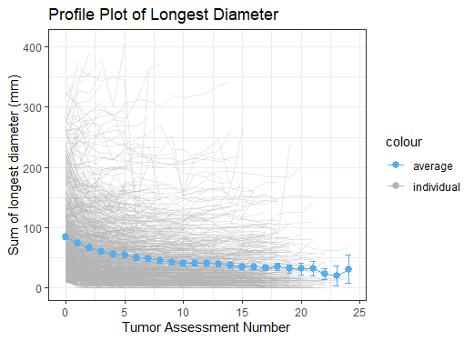
\includegraphics[width=0.55\textwidth]{chapters/figures/profile_LD.png}\label{fig:profile_LD}}
    \hfill
    \subfloat[]{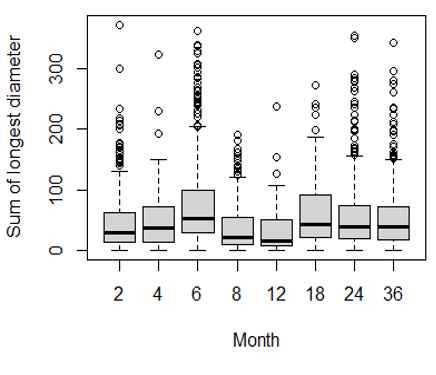
\includegraphics[width=0.45\textwidth]{chapters/figures/box_LD.png}\label{fig:box_LD}}
    \caption{Profile plot and boxplot of the sum of the longest diameter of target lesions}
\end{figure}

This research was motivated by a phase 3, randomized, open-label, parallel-arm study that compared an experimental drug with the standard of care (As the trial data is currently not accessible to the public, we are unable to provide further information about the trial at this time). A total of 798 treatment-naive adult participants with advanced renal cell carcinoma were randomized (1:1) to receive either the experimental drug or the active comparator. Additional key inclusion criteria were the presence of at least one measurable lesion defined by \acs{RECIST} version 1.1 that had not been previously irradiated. Tumor assessments were performed using computed tomography or magnetic resonance imaging at baseline, every six weeks after randomization for the first 18 months, and then every 12 weeks until confirmed disease progression. Baseline demographic and disease characteristics were balanced between the two treatment groups. The two primary endpoints were \ac{PFS} and \ac{OS} among patients with programmed death ligand 1 (PD-L1)–positive tumors. This trial concluded that patients who received the experimental drug had significantly longer \ac{PFS} than patients who received the active comparator. As of the cutoff date of our obtained dataset, 335 (42\%) deaths were observed, and the corresponding subject-specific profile plot and box plot of target lesion measurements are shown in Figure \ref{fig:profile_LD} and \ref{fig:box_LD}. Notice that there is significant between-individual variability in the trajectories of the sum of the longest diameter over time in Figure \ref{fig:profile_LD}. Therefore, it is necessary to consider random effects when modeling target lesion measurements. The Kaplan-Meier plot of non-target lesions and new lesions are shown in Figure \ref{fig:NT_KMplot} and \ref{fig:NL_KMplot}. We observe a difference between the two treatment arms from both plots: patients who received the experimental drug had a longer time to \ac{PD} considering non-target lesion and new lesion assessments.

\begin{figure}[ht]
    \centering
    \subfloat[]{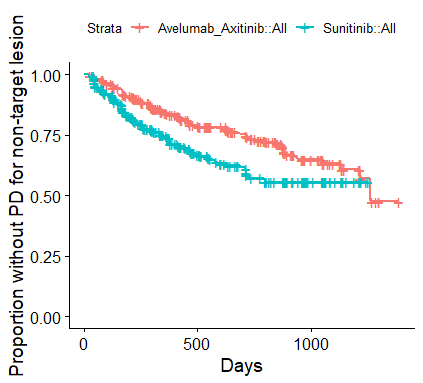
\includegraphics[width=0.5\textwidth]{chapters/figures/NT_KMplot.png}\label{fig:NT_KMplot}}
    \hfill
    \subfloat[]{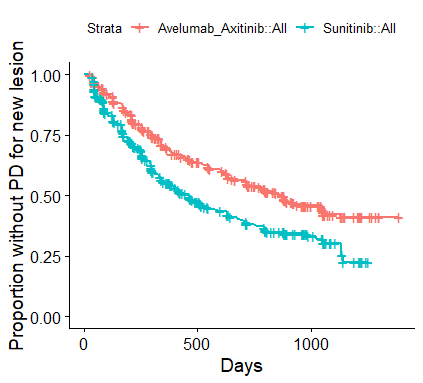
\includegraphics[width=0.5\textwidth]{chapters/figures/NL_KMplot.png}\label{fig:NL_KMplot}}
    \caption{Kaplan-Meier plots of time to progressive design considering non-target lesions (a) and new lesions (b)}
\end{figure}

Our goal in this study is to use the observed data to construct a predictive tool that provides a reliable estimate of the time of the $n$th death in the trial. Specifically, we will use data on participants' baseline characteristics, treatment group, \ac{OS}, target lesion measurements, and the progression of disease of non-target lesions and new lesions. Note, a participant who has the $n$th death does not mean this participant survived the $n$th longest among all trial participants, as the time of $n$th death is calculated by adding the participant's \ac{OS} to their randomization date.

\section{Method}
\label{sec:method}

\subsection{Standard Statistical Analysis}
The standard method of analysis of \ac{PFS} includes using a Kaplan-Meier curve or Cox regression. A patient who progresses or dies during the study is considered an event in the analysis. For trial participants, the event time is defined as the duration between the randomization date and the earliest date when \ac{PD} (by any of the four processes) is observed. If a participant does not have an event during the study, they are censored at the last visit when they had an adequate disease assessment.

The major caveat of this measurement of \ac{PFS} is that it does not consider the dynamics of the four component processes of \ac{PFS}: 1) measurement of target lesion (longitudinal continuous data), 2) time to non-target lesion progression (time to event endpoint), 3) time to new lesion (time to event endpoint), and 4) death (time to event endpoint). Given that the growth of the tumors considered in these processes is not independent of each other, we propose a joint modeling approach that captures the change in different types of tumor measurements to assess more of the component processes in \ac{PFS}. 

\subsection{Multivariate Joint Modeling Approach}
\label{sec:jm}

In this section, we set up each of three joint models between each of the processes that make \ac{PFS} and \ac{OS}, along with the marginal model for \ac{OS}. By applying \ac{BMA}, we obtain the final predicted probability of \ac{OS}. The structure of the proposed multivariate joint modeling approach is illustrated in Figure \ref{fig:JM} where details follow below in each subsection.

\subsubsection{Model for the Association between Target Lesion and OS}

We consider a set of n subjects followed over an interval [0,$\tau$]. Let $z_{ij}$ be the target lesion measurement (or \% change from baseline) at time $t_{ij}$ (for the $i$-th participant at the $j$-th visit) where $i=1,...,n$ and $j=1,...,k_i$. We assume the target lesion measurement time $t_{ij}$ is non-informative so that it is independent of the longitudinal measurement and event-time processes for \ac{OS}. We define a latent zero-mean Gaussian process $W_i(t)$ for the $i$-th participant, independent of different participants. The following sub-models link the joint model of lesion measurements and \ac{OS}:

The observed lesion measurement
$$Y_{i}(t)=\mu_{i}(t)+\epsilon_i$$
where the lesion measurement process $\mu_{i1}$, $\mu_{i2}$,...
is modeled by the linear model
$$\mu_{i}(t)=\textbf{X}_i(t)' \boldsymbol{\beta}_{\mu}+W_{i}(t)$$
where $\textbf{X}_i(t)$ is the time-dependent covariate matrix for subject $i$'s lesion measurement and $\epsilon_i$ is the measurement error. $W_i(t)$ is a Gaussian process that has the following form,
$$W_{1i}(t)=b_{1i}+b_{2i}*t$$
where ($b_{1i},b_{2i}$) are zero-mean bivariate Gaussian variables with variances $\sigma_1^2$ and $\sigma_2^2$ respectively, and correlation coefficient $\rho$. 

The \ac{OS} process at time t is modeled by
$$\lambda(t)=\lambda_0(t) \exp(\textbf{Z}_i' \boldsymbol{\beta}_{\rm OS}+\lambda \mu_{i}(t)+b_{3i})$$
Under the Weibull baseline hazard, $\lambda(t)$ has the following form
$$\lambda(t)=\alpha_{\rm OS,TL} \gamma_{\rm OS} t^{\alpha_{\rm OS,TL}-1} \exp(\textbf{Z}_i' \boldsymbol{\beta}_{\rm OS}+\lambda \mu_{i}(t)+b_{3i})$$
where $\textbf{Z}_i$ is the covariate matrix for \ac{OS} and $b_{3i}\sim N(0,{\sigma_3})^2$ models random effect orthogonal to the measurement process. 

The marginal distribution of the observed measurements $\mu$ is easily obtained. The likelihood for the observed data can be factorized as the product of this marginal distribution and the conditional distribution of \ac{OS}, given the observed values of $\mu$. Let $\boldsymbol{\theta}_1$ denote the combined vector of unknown parameters. Conditional on lesion measurement $\mu$, \ac{OS} is independent of the measurements $\mu$, so we can write the likelihood $L=L(\boldsymbol{\theta}_1, \mu, OS)$ as
$$
L=L_{\mu}(\boldsymbol{\theta}_1,\mu)  \times L_{OS| \mu}(\boldsymbol{\theta}_1,OS|\mu)
$$
where $L_{\mu}(\boldsymbol{\theta}_1,\mu)$ is of standard form corresponding to the marginal multivariate normal distribution of $\mu$ and
$$
L_{OS|\mu}(\boldsymbol{\theta}_1, OS|\mu)=\prod_i \bigg\{ \bigg[\lambda_0 (t) \exp(\textbf{Z}_i' \boldsymbol{\beta}_{\rm OS}+\lambda \mu_{i}(t)) \bigg]^{\delta_{OS,i}}
$$

$$
\times \exp \bigg[ -\int_0^{y_{OS,i}} \lambda_0(t) \exp(\textbf{Z}_i' \boldsymbol{\beta}_{\rm OS}+\lambda \mu_{i}(t))dt\bigg]\bigg\}
$$
where $y_{OS,i}=\min(t_{OS,i},c_{OS,i})$ and $\delta_{OS,i}=I(t_{OS,i}\leq c_{OS,i})$. $c_{OS,i}$ is the censoring time for the $i$th participant and $t_{OS,i}$ is the true event time.


%
%\begin{eqnarray*}
%z_{ij} = \mbox{\boldmath{$X$}}'\mbox{\boldmath{$\beta_{z}$}} + b_{1i} + b_{2i}*t_{ij}
%\end{eqnarray*}
%
%where $i= 1,\ldots,n$ and $j= 1, \ldots,k_{i}$.
%
%\begin{eqnarray*}
%\lambda(t_{OS}) = \lambda_{0}(t_{OS})\exp({\mbox{\boldmath{$X$}}'\mbox{\boldmath{$\beta_{os}$}} + z_{ij}})
%\end{eqnarray*}
%
%{\color{red}
%\begin{itemize}
%\item There is a positivity probability that $z_{ij}$ can be 0 (or -100\% for \% change). Should we model that probability?
%\item Do we need to model the skewness in longitudinal data?
%\end{itemize}
%}


\subsubsection{Model for Time to Non-Target Lesion and OS}
Let $t$ be the time from the initial treatment until the occurrence
of an event, i.e., non-target lesion or a new lesion, and let $\textbf{Z}$ be covariates of interest.
For a participant with covariates $\textbf{Z}$, let $\lambda_{\rm NT}(t|\textbf{Z})$
denote the hazard function for the time to non-target lesion progression. Under the Cox
proportional hazards model, we have
\begin{equation*}
\lambda_{\rm NT}(t|\textbf{Z})=\lambda_{0, \rm NT}(t)\mathrm{exp}(\textbf{Z}' \boldsymbol{\beta_{\rm NT}}). \label{cox}
\end{equation*}
When the baseline hazard $\lambda_{0, \rm NT}(t)$ is modeled by a Weibull
distribution, the corresponding survival function is given by
\begin{equation}
S_{\rm NT}(t|\textbf{Z})=\mathrm{exp}\{-\gamma_{\rm NT} t^{\alpha_{\rm NT}}
\mathrm{exp}(\textbf{Z}' \boldsymbol{\beta_{\rm NT}} )\},\label{SurvT}
\end{equation}
such that $\gamma_{\rm NT}$ and $\alpha_{\rm NT}$ are the scale and shape parameters
of the Weibull distribution, respectively. Similarly, we
model $S_{\rm NL}(t|\textbf{Z})$ by the proportional hazards model with a Weibull baseline hazard:
\begin{equation}
S_{\rm NL}(t|\textbf{Z})=\mathrm{exp}\{-\gamma_{\rm NL} t^{\alpha_{\rm NL}}
\mathrm{exp}(\textbf{Z}' \boldsymbol{\beta_{\rm NL}} )\}. \label{SurvE}
\end{equation}
For \ac{OS},
\begin{equation}
S_{\rm OS}(t|\textbf{Z})=\mathrm{exp}\{-\gamma_{\rm OS} t^{\alpha_{\rm OS}}
\mathrm{exp}(\textbf{Z}' \boldsymbol{\beta_{\rm OS}} )\}. \label{SurvOS}
\end{equation}

To take into account the heterogeneity of the patient population, we introduce random effects for the shape parameter of the Weibull model denoted as $b_{NT_i}$, $b_{NL_i}$, and $b_{OS_i}$. Then we have
$$\alpha_{NT_i}=\alpha_{NT}+b_{NT_i}$$
$$\alpha_{NL_i}=\alpha_{NL}+b_{NL_i}$$
$$\alpha_{OS_i}=\alpha_{OS}+b_{OS_i}$$

Furthermore, it is critical to take into account the correlations
between times to non-target lesion progression and \ac{OS} and new lesion and \ac{OS}. We achieve this by using the \cite{clayton1978model} model to model the bivariate time-to-event data as
\begin{equation}
S_1(t_{\rm NT},
t_{\rm OS}|\textbf{Z})=\{S_{\rm NT}(t_{\rm NT}|\textbf{Z})^{-\eta_{\rm NT}}
+S_{\rm OS}(t_{\rm OS}|\textbf{Z})^{-\eta_{\rm NT}}-1\}^{-1/\eta_{\rm NT}}, \label{clayton1}
\end{equation}
where $t_{\rm NT}$ and $t_{\rm OS}$ denote times to non-target lesion progression and \ac{OS} (death),
respectively, and $\eta_{\rm NT}>0$ measures their correlation.
The relationship between Kendall's $\tau$ and the correlation parameter $\eta_{\rm NT}$
is $\tau_{\rm NT} = \eta_{\rm NT}/(2+\eta_{\rm NT})$. A large value of $\eta_{\rm NT}$
represents a high correlation. When $\eta$ goes to 0,
the correlation approaches 0, and when $\eta_{\rm NT}$ goes to $\infty$, the correlation converges to 1.
For non-target lesions,
define $y_{\rm NT}=\mathrm{min}(t_{\rm NT}, c_{\rm NT})$ and
$\delta_{\rm NT}=I(t_{\rm NT} \le c_{\rm NT})$,
where $c_{\rm NT}$ and $I(\cdot)$ denote the censoring time and the indicator function,
respectively; and define $y_{\rm OS}$ and $\delta_{\rm OS}$ similarly for \ac{OS}.

Depending on the censoring pattern, the observed date for the $i$th participant falls into one of the
following mutually exclusive cases:

\begin{itemize}
\item Case 1: Both $t_{NT}$ and $t_{OS}$ are observed. ($\delta_{NT}$=1, $\delta_{OS}$=1)
\item Case 2: $t_{NT}$ is observed and $t_{OS}$ is censored. ($\delta_{NT}$=1, $\delta_{OS}$=0)
\item Case 3: $t_{NT}$ is censored and $t_{OS}$ is observed. ($\delta_{NT}$=0, $\delta_{OS}$=1)
\item Case 4: Both $t_{NT}$ and $t_{OS}$ are censored. ($\delta_{NT}$=0, $\delta_{OS}$=0)

\end{itemize}

Let
$\boldsymbol{\theta}_2=(\boldsymbol{\beta_{\rm NT}}, \alpha_{\rm NT_i}, \lambda_{\rm NT}, \boldsymbol{\beta_{\rm OSNT}},
\alpha_{\rm OSNT_i}, \lambda_{\rm OS}, \eta_{\rm NT})$,  then the
likelihood for the $i$th patient with ${\rm Data}_i=(y_{\rm NT}, y_{\rm OS},
\delta_{\rm NT}, \delta_{\rm OS}, \textbf{Z})_i$ is given by
$$
L(\boldsymbol{\theta}_2|{\rm Data}_i)
=L_1^{\delta_{\rm NT}\delta_{\rm OS}}
L_2^{\delta_{\rm NT}(1-\delta_{\rm OS})}L_3^{(1-\delta_{\rm NT})\delta_{\rm OS}}
L_4^{(1-\delta_{\rm NT})(1-\delta_{\rm OS})}, \label{likelihood1}
$$

where
$L_1=\frac{\partial^2\, S_1(t_{\rm NT}, t_{\rm OS}|\textbf{Z})}{\partial t_{\rm NT} \partial t_{\rm OS}}\big|_{t_{\rm NT}=y_{\rm NT},t_{\rm OS}=y_{\rm OS}}$, $L_2=-\frac{\partial S_1(t_{\rm NT}, t_{\rm OS}|\textbf{Z})}{\partial t_{\rm NT}}\bigg|_{t_{\rm NT}=y_{\rm NT},t_{\rm OS}=y_{\rm OS}}$, $L_3=-\frac{\partial S_1(t_{\rm NT}, t_{\rm OS}|\textbf{Z})}{\partial t_{\rm OS}}\bigg|_{t_{\rm NT}=y_{\rm NT},t_{\rm OS}=y_{\rm OS}}$, and $L_4=S_1(t_{\rm NT}, t_{\rm OS}|\textbf{Z})\bigg|_{t_{\rm NT}=y_{\rm NT},t_{\rm OS}=y_{\rm OS}}$.

%\begin{eqnarray*}
%L_1 &=& \frac{\partial^2\, S(y_{\rm NT}, y_{\rm OS}|\textbf{Z})}
%{\partial y_{\rm NT} \partial y_{\rm OS}} \\
%L_2 &=& -\frac{\partial S(y_{\rm NT}, y_{\rm OS}|\textbf{Z})}
%{\partial y_{\rm NT}} \\
%L_3 &=& S(y_{\rm NT}, y_{\rm OS}|\textbf{Z}).
%\end{eqnarray*}

For a given subject, $L_1, L_2$,  $L_3$ and $L_4$ correspond to the likelihood components that both non-target lesion and \ac{OS} are observed, non-target lesion is observed but \ac{OS} is censored, non-target lesion is censored but \ac{OS} is observed, and both non-target lesion and \ac{OS} are censored, respectively. The derivation of $L_1$, $L_2$, $L_3$, and $L_4$ are provided in the supplementary materials of this manuscript. 


%\begin{eqnarray}

%\end{eqnarray}


\subsubsection{Model for Time to New Lesion and OS}
Similarly, for the relationship between time to new lesion and \ac{OS}, we model
the bivariate time-to-event data using the \cite{clayton1978model} model,
\begin{equation}
S_2(t_{\rm NL},
t_{\rm OS}|\textbf{Z})=\{S_{\rm NL}(t_{\rm NL}|\textbf{Z})^{-\eta_{\rm NL}}
+S_{\rm OS}(t_{\rm OS}|\textbf{Z})^{-\eta_{\rm NL}}-1\}^{-1/\eta_{\rm NL}}. \label{clayton2}
\end{equation}
Let
$\boldsymbol{\theta}_3=(\boldsymbol{\beta_{\rm NL}}, \alpha_{\rm NL_i}, \lambda_{\rm NL}, \boldsymbol{\beta_{\rm OSNL}},
\alpha_{\rm OSNL_i}, \lambda_{\rm OS}, \eta_{\rm NL})$,  then the likelihood for the $i$th patient with ${\rm Data}_i=(y_{\rm NL}, y_{\rm OS},
\delta_{\rm NL}, \delta_{\rm OS}, \textbf{Z})_i$ is given by
$$
L(\boldsymbol{\theta}_3|{\rm Data}_i)
=L_1^{\delta_{\rm NL}\delta_{\rm OS}}
L_2^{\delta_{\rm NL}(1-\delta_{\rm OS})}L_3^{(1-\delta_{\rm NL})\delta_{\rm OS}}
L_4^{(1-\delta_{\rm NL})(1-\delta_{\rm OS})}, \label{likelihood2}
$$

where $L_1=\frac{\partial^2\, S_2(t_{\rm NL}, t_{\rm OS}|\textbf{Z})}{\partial t_{\rm NL} \partial t_{\rm OS}}\big|_{t_{\rm NL}=y_{\rm NL},t_{\rm OS}=y_{\rm OS}}$, $L_2=-\frac{\partial S_2(t_{\rm NL}, t_{\rm OS}|\textbf{Z})}{\partial t_{\rm NL}}\bigg|_{t_{\rm NL}=y_{\rm NL},t_{\rm OS}=y_{\rm OS}}$, $L_3=-\frac{\partial S_2(t_{\rm NL}, t_{\rm OS}|\textbf{Z})}{\partial t_{\rm OS}}\bigg|_{t_{\rm NL}=y_{\rm NL},t_{\rm OS}=y_{\rm OS}}$, and $L_4=S_1(t_{\rm NL}, t_{\rm OS}|\textbf{Z})\bigg|_{t_{\rm NL}=y_{\rm NL},t_{\rm OS}=y_{\rm OS}}$.
The derivation of $L_1$, $L_2$, $L_3$, and $L_4$ can also be found in the supplementary materials.

\subsubsection{Model for OS}
We model \ac{OS} with a simple Weibull baseline hazard model that has the following form
$$\lambda(t)=\alpha_{\rm OS,M} \gamma_{\rm OS} t^{\alpha_{\rm OS,M}-1} \exp(\textbf{Z}_i' \boldsymbol{\beta_{M}})$$
where $\textbf{Z}_i$ is the covariate matrix for modeling \ac{OS}.

Now that we have defined the three models for the relationships between the target lesion, non-target lesion, and new lesion and \ac{OS} and the marginal model of \ac{OS}, we can take a \ac{BMA} approach to link all four models
for better prediction.

\subsubsection{Bayesian Model Average and Prediction}

Denote the above three joint models and one marginal model for \ac{OS} by $M_T$, $M_{NT}$, $M_{NL}$, and $M_{OS}$, respectively. Then by \ac{BMA}, the final predicted probability of \ac{OS} follows
$$P(Y_{pred}|Data)=P(Y_{pred.t}|M_T,Data)P(M_T|Data)$$
$$+P(Y_{pred.nt}|M_{NT},Data)P(M_{NT}|Data)+P(Y_{pred.nl}|M_{NL},Data)P(M_{NL}|Data)$$
$$+P(Y_{pred.os}|M_{OS},Data)P(M_{OS}|Data)$$
where $P(M_T|Data)$, $P(M_{NT}|Data)$, $P(M_{NL}|Data)$, and $P(M_{OS}|Data)$ are the model weights. In general, if we have a total of $Q$ models, the model weight for model $q$ at the $t$th MCMC iteration is  
$$w^{(t)}_q=P(M_q|Data,\theta^{(t)})=\frac{P(M_q,Data,\theta^{(t)})}{P(Data,\theta^{(t)})}$$
$$=\frac{P(Data|M_q,\theta^{(t)})P(\theta^{(t)}|M_q)P(M_q)}{P(Data,\theta^{(t)})}$$
where $\theta^{(t)} = (\theta_1^{(t)}, \theta_2^{(t)},...,\theta_Q^{(t)})$. If we set $P(\theta_h|M_h, Data)=g_h$, and $q \ne h$, then according to \cite{congdon2007model},
$$P(\theta^{(t)}|M_q)=P(\theta_q^{(t)}|M_q) \prod_{h=1,h\ne q}^Q P(\theta_h^{(t)}|M_q)=P(\theta_q^{(t)}|M_q) \prod_{h=1,h\ne q}^Q g_h$$.
Therefore, 
$$w^{(t)}_q=P(M_q|Data,\theta^{(t)})$$
$$
=\frac{P(Data|M_q,\theta^{(t)}_q) P(\theta^{(t)}_q|M_q) \prod_{h=1,h\ne q}^Q g_h P(M_q)}{\sum_{k=1}^Q P(M_k,Data, \theta^{(t)})} 
$$
$$=\frac{P(Data|M_q,\theta^{(t)}) P(\theta_q^{(t)}|M_q) \prod_{h=1,h\ne q}^Q g_h P(M_q) }{\sum_{k=1}^Q P(Data|M_k,\theta^{(t)}) P(\theta_k^{(t)}|M_k) \prod_{h=1,h\ne k}^K g_h P(M_k)}.
$$
Through the above formula, we implement the \ac{BMA} approach and calculate the final predicted \ac{OS}. 

\begin{figure}[ht]
\centering
\subfloat[]{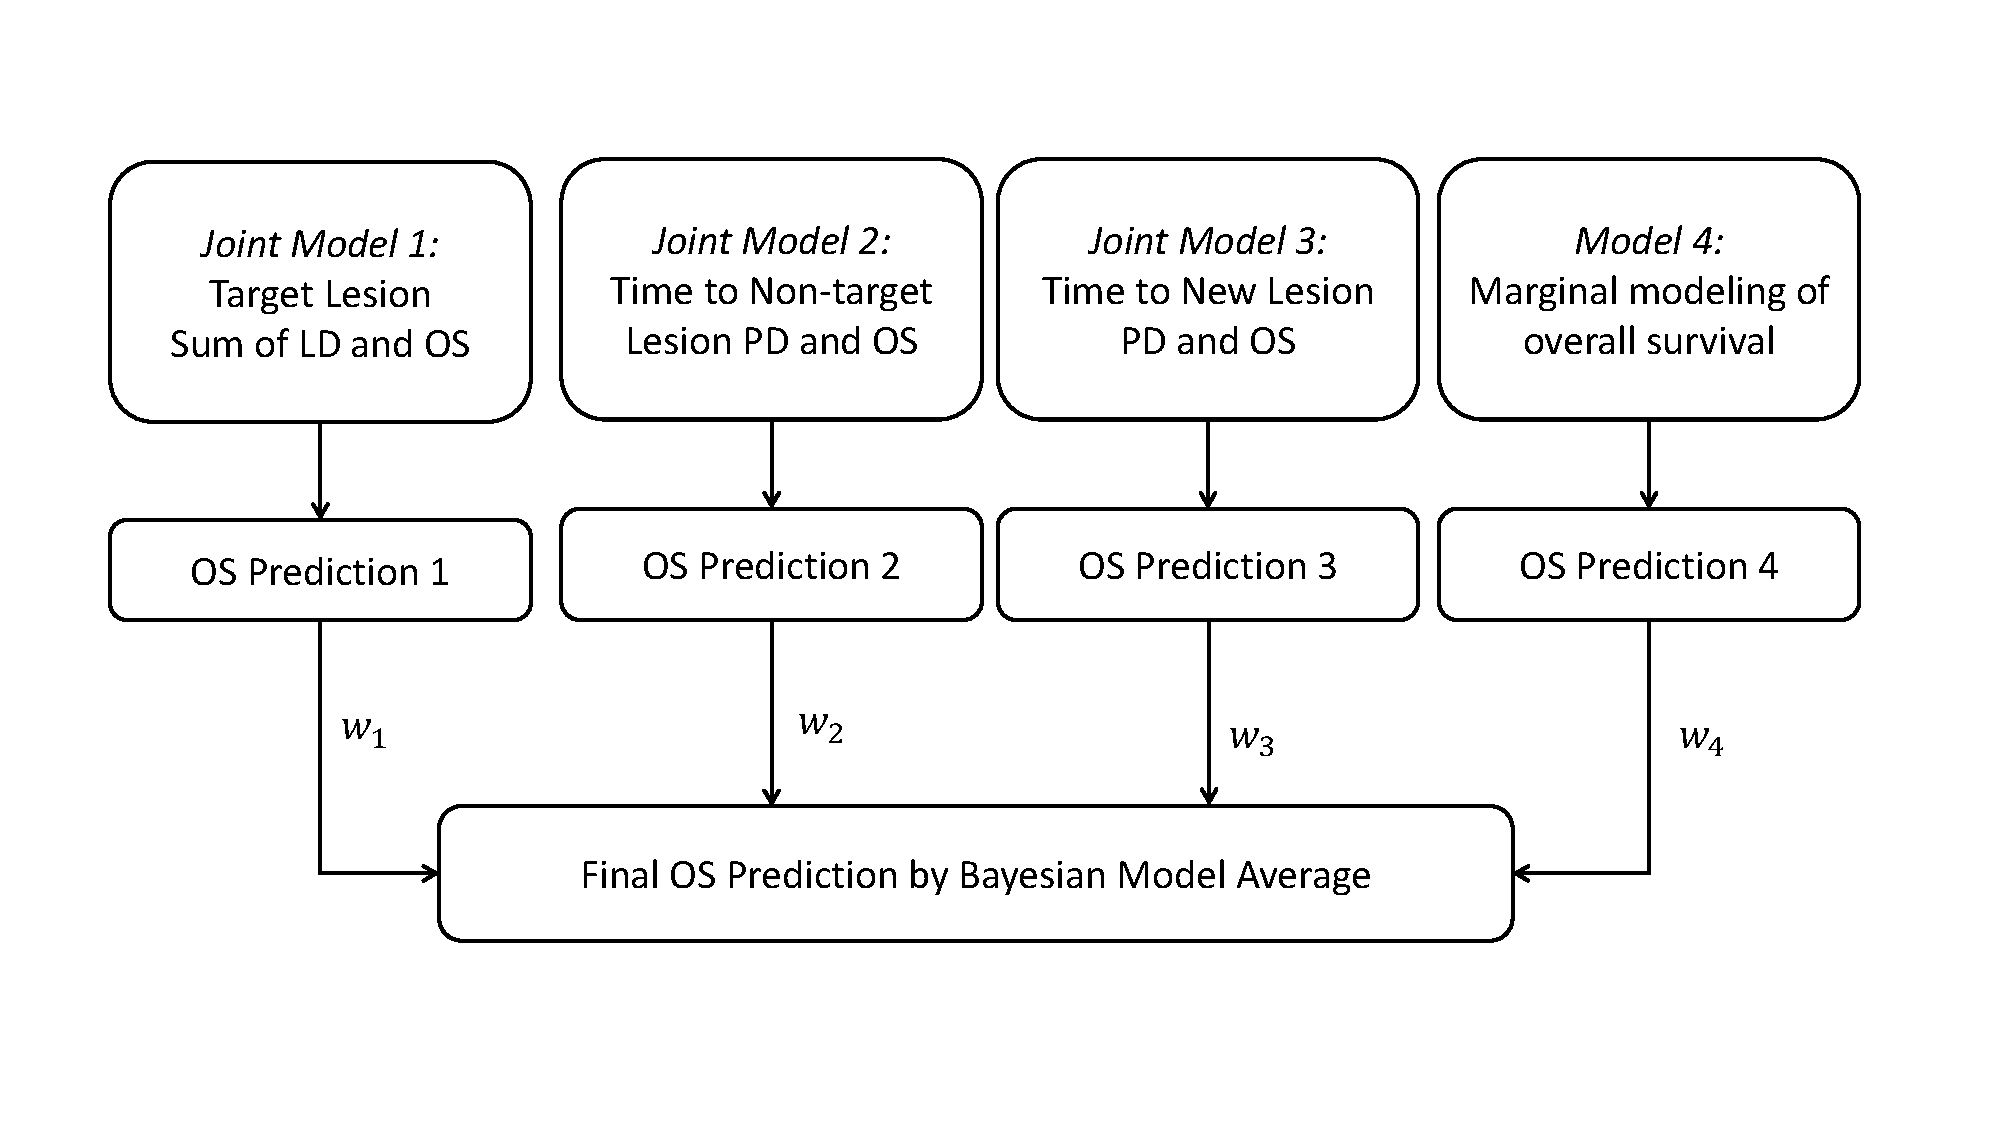
\includegraphics[width=\textwidth]{chapters/figures/JM.pdf}\label{fig:JM}}
\\
\subfloat[]{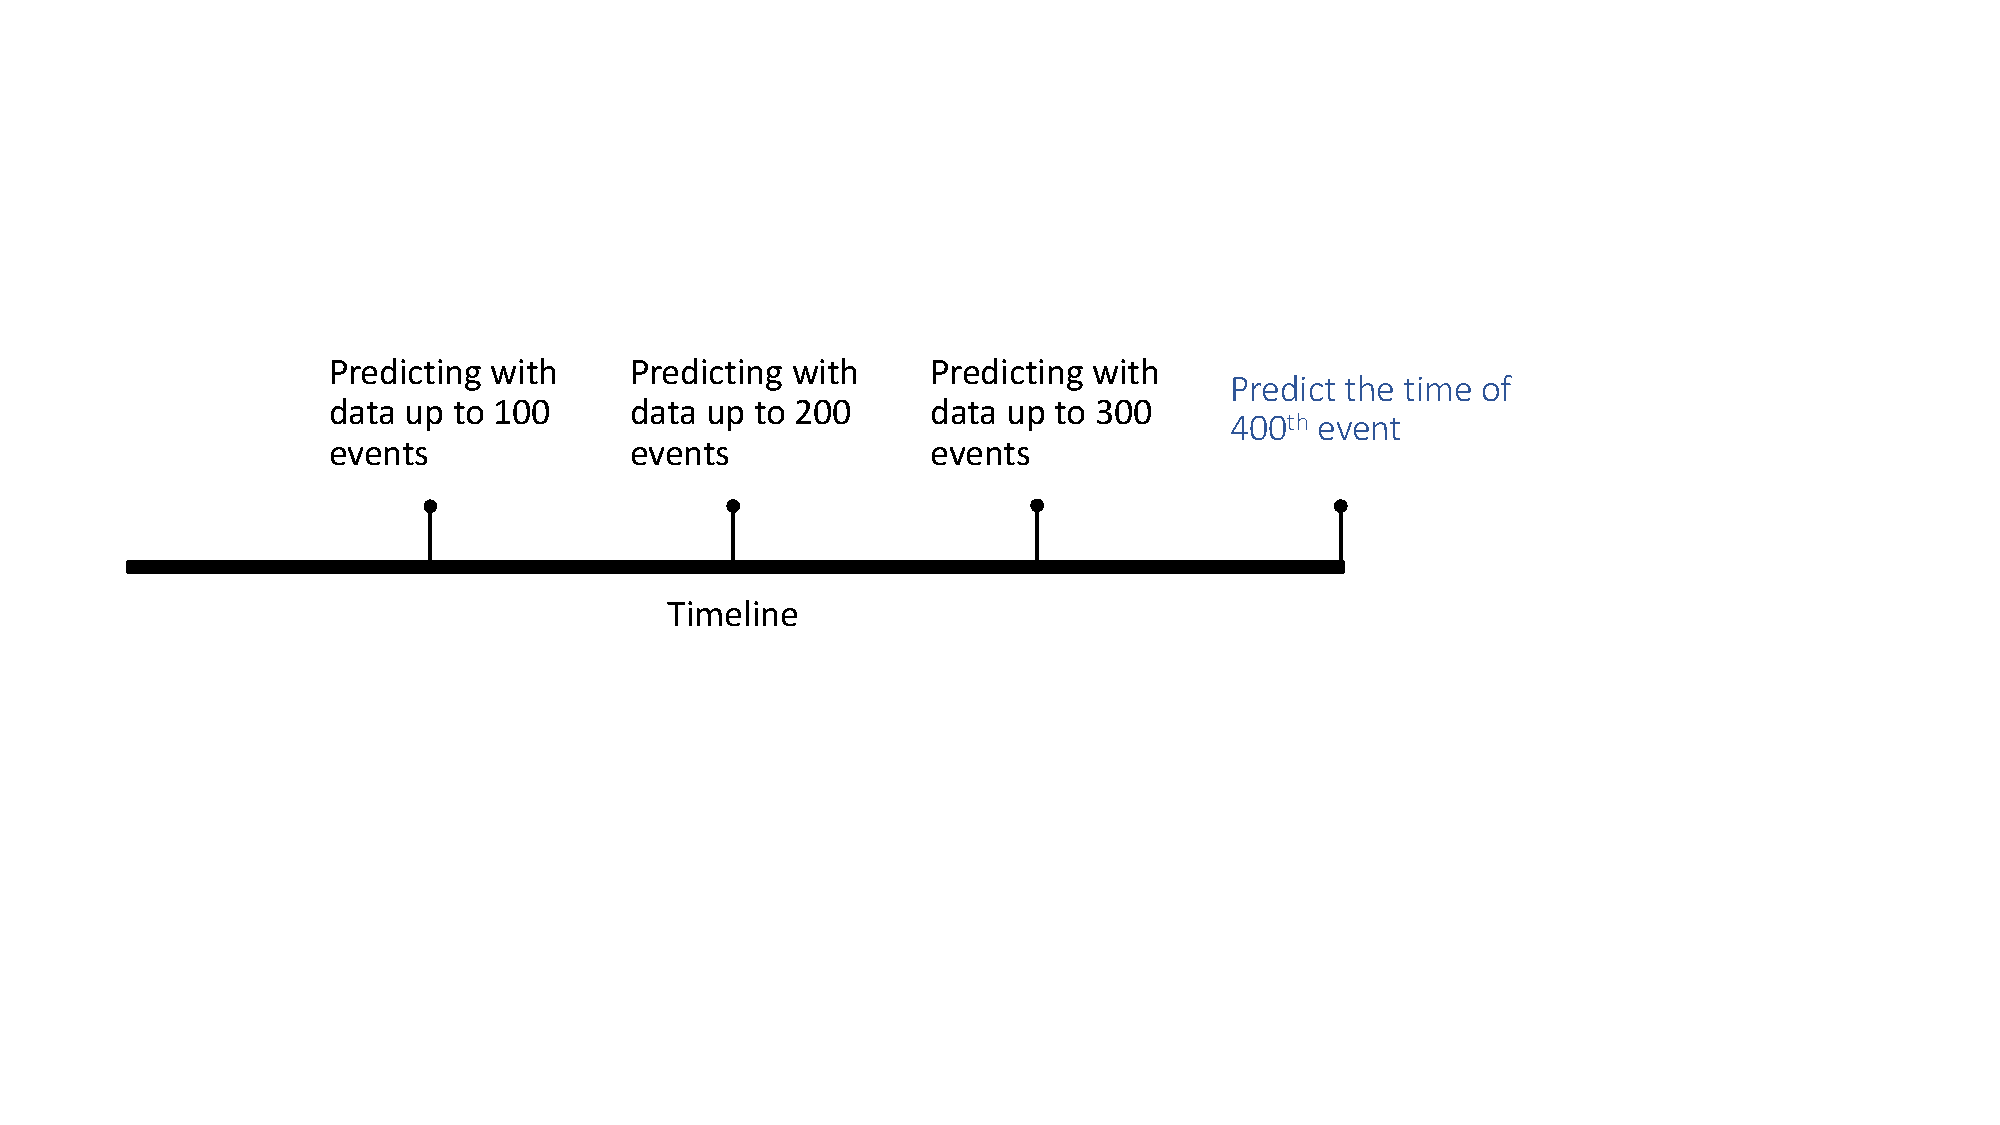
\includegraphics[width=\textwidth]{chapters/figures/timeline.pdf}\label{fig:timeline}}
\caption{(a) Multivariate joint modeling structure. (b) Predict the time of last (400th) event with observed data up to 100/200/300 events.}
\end{figure}

\subsubsection{Prior Specification}
We suggest weakly informative normal distributions with mean 0 as priors for $\boldsymbol{\beta_{\mu}}$, $\boldsymbol{\beta_{OS}}$, $\boldsymbol{\beta_{NT}}$, $\boldsymbol{\beta_{OSNT}}$, $\boldsymbol{\beta_{NL}}$, $\boldsymbol{\beta_{OSNL}}$ and $\boldsymbol{\beta_{M}}$, exponential distributions with rates equal to 1 or 0.5 as priors for $\alpha_{NT}$, $\alpha_{NL}$, $\alpha_{OS,TL}$, $\alpha_{OSNT}$, $\alpha_{OSNL}$, $\alpha_{OS,M}$, $\eta_{NT}$ and $\eta_{NL}$, and a weakly informative normal distribution with mean 0 as prior for $\lambda$. For the correlation coefficient $\rho$, we recommend non-informative prior $Unif(-1, 1)$. Random effects $b_{1i}$, $b_{2i}$, $b_{3i}$, $b_{NT_i}$, $b_{NL_i}$, $b_{OSNT_i}$ and $b_{OSNL_i}$ follow normal distribution $N(0, \sigma_{b_k}^2)$, where $k = 1i, 2i, 3i, NT_i, NL_i, OSNT_i, OSNL_i$, respectively. We suggest half-normal priors with standard deviations equal to 1 for all $\sigma_{b_{k}}$. In addition, we assume that all models are equally weighted before fitting \ac{BMA}, that is, $P(M_q) = 1/Q$, for all $q = 1,...,Q$.

\section{Simulation}
\label{sec:simulation}

\subsection{Design}
We performed extensive simulations to evaluate the performance of the proposed multivariate joint modeling approach. All simulated datasets mimic the structure of the renal cell cancer trial data. Specifically, we assume 400 subjects and 25 visits. Longitudinal measurements of target lesion and new lesion status are recorded at each visit. For simplicity purposes, non-target lesion status is not included. Survival status also gets updated whenever deaths occur. The follow-up visits are scheduled for every two months within the first two years, then change to every three months until the end of the 5th year. We censor the subject's subsequent target lesion measurements and new lesion status whenever that subject's death occurs. In addition, we have assumed three scenarios: 1) \ac{OS} is independent of target lesion measurements and time to new lesion, 2) \ac{OS} is correlated with time to new lesion only, and 3) \ac{OS} is correlated with target lesion measurements only. In all scenarios, target lesion measurements and new lesion status are randomly and independently simulated, but \ac{OS} is generated under different conditions. Specifically, in scenario 1, \ac{OS} is randomly and independently simulated. In scenario 2, \ac{OS} is conditionally simulated from a bivariate copula model between \ac{OS} and new lesion status. Finally, in scenario 3, \ac{OS} is conditionally simulated based on the target lesion measurements. We assume a negative correlation between \ac{OS} and changes in tumor measurements. For each scenario, 200 datasets are generated. To simplify the simulation process, only $treatment$ is included in the covariate matrices. 

We compare predictions under three models: our proposed multivariate joint model, a copula model for \ac{PFS} and \ac{OS}, and a marginal Weibull baseline hazard model of \ac{OS}. The copula model for \ac{PFS} and \ac{OS} follows exactly the same structure as the copula model for non-target lesion/new lesion and \ac{OS}, where the variables with NT/NL subscripts are replaced by the subscripts corresponding to \ac{PFS}. 

To emulate real trial scenarios and assess the prediction performance of our proposed method, we generate snapshots of the data such that for each simulated dataset, we have snapshots of what the data would have looked like if only 100, 200, and 300 death events had occurred (Figure \ref{fig:timeline}). Then, we predict the time of the last (400th) death event under each snapshot dataset. Note that predictions may be performed at any time during the trial, and 100, 200, and 300 are selected for illustration purposes. Predictions from the three methods are compared. Finally, we calculate each predictor's \ac{CR}, \acl{rMSE} (\acs{rMSE}), bias, and width of the 90\% \acl{CI} (\acs{CI}). The 90\% \ac{CI} is the narrowest interval that includes 90\% of the posterior distribution of the predictor. 

\subsection{Results}

\begin{figure}[t]
\centering
\subfloat[]{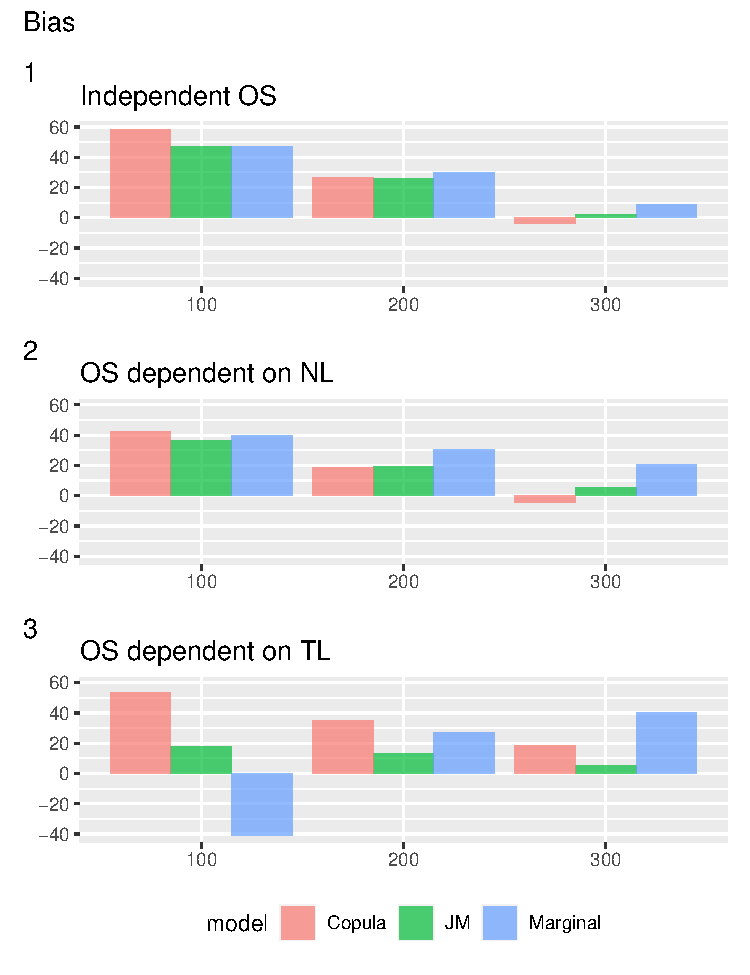
\includegraphics[width=0.5\textwidth]{chapters/figures/osbma-Bias.pdf}\label{fig:bias}}
\subfloat[]{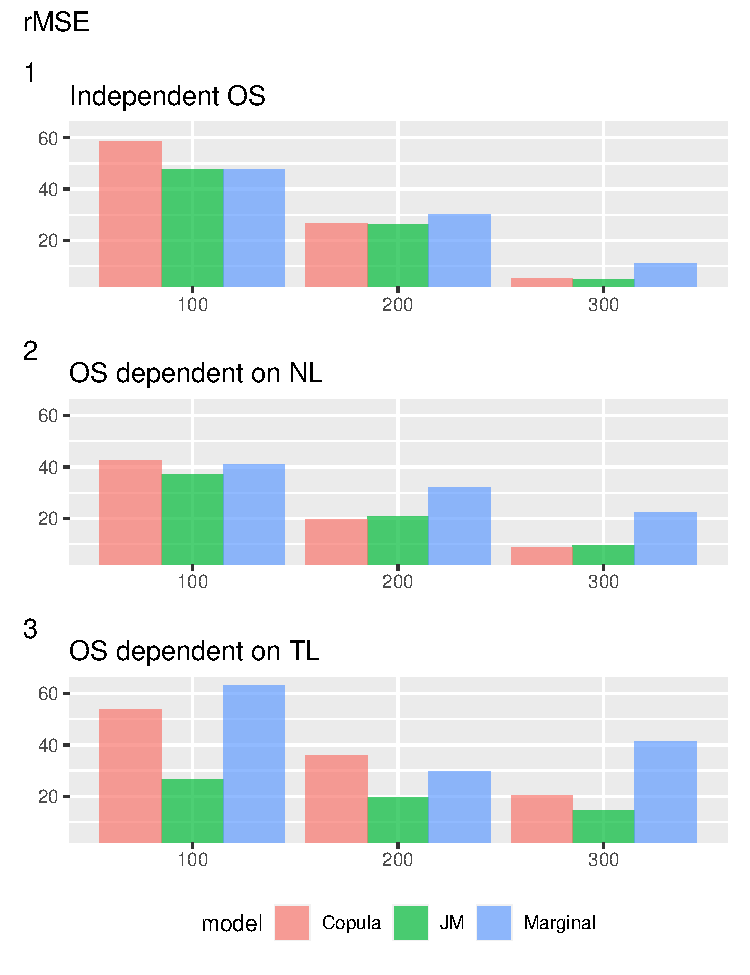
\includegraphics[width=0.5\textwidth]{chapters/figures/osbma-rMSE.pdf}\label{fig:rmse}}
\caption{The bias (a) and rMSE (b) of the predictors of three models: the multivariate joint modeling approach (JM), a copula model between PFS and OS (Copula), and the marginal Weibull baseline hazard model of OS (Marginal), under three OS scenarios. The $x$-axis denotes the number of death at cutoff. The $y$-axis denotes the number of months. \label{fig:result}}
\end{figure}

The bias and \ac{rMSE} of the predicted time of the last death are shown in Figures \ref{fig:bias} and \ref{fig:rmse}, and the corresponding \ac{CR} and \ac{CI} width are shown in Supplementary Table 1. 

Under scenario 1, where \ac{OS} is generated independently, the bias and \ac{rMSE} of all predictors become smaller as we gather more information from the trial, i.e., more death events are observed. The marginal model performs the worst when we observe 200 or 300 death events, which is most likely caused by not incorporating random effects in the model. Even though the copula model and the multivariate joint modeling approach have very similar bias and \ac{rMSE} when 200 or 300 death events are observed, the \ac{CI} widths of the multivariate joint modeling approach are smaller. Having evaluated all the metrics, the marginal joint modeling approach is the best-performing method under scenario 1.

Under scenario 2, where \ac{OS} is generated conditional on new lesion status, the copula model has the smallest bias and \ac{rMSE} when a reasonable amount of death events have been observed. In our simulations, 200 (50\%) death events are more than enough for the copula model to show its advantages. Similar to scenario 1, as more death events are observed, the bias and \ac{rMSE} of all predictors become smaller. Compared to the multivariate joint modeling approach, the slightly smaller bias and \ac{rMSE} values of the copula model are very likely attributable to directly modeling the relationship between \ac{PFS} and \ac{OS}, where \ac{PFS} also has death as one of its components. Whereas the differences in bias and \ac{rMSE} are negligible, the copula model has significantly bigger \ac{CI} widths than the other two methods. Overall, we would still recommend the marginal joint modeling approach under scenario 2.

Under scenario 3, where \ac{OS} is generated conditional on the target lesion measurements, the proposed multivariate joint modeling approach performs significantly better than the other two models. This is unsurprising as the multivariate joint modeling approach is the only method that captures the relationship between \ac{OS} and the target lesion. Unlike the other two scenarios, the bias and \ac{rMSE} of the predictors from the marginal model do not always decrease when more death events are observed. This is due to the large survival time simulated under scenario 3 and the inflexibility of the standard Weibull baseline hazard model without random effects. 

According to Figure \ref{fig:result}, across all scenarios, the proposed multivariate joint modeling approach performs either the best or very similar to the better model among the remaining two. This is reasonable as the \ac{BMA} could assign $w_q = 1$ to submodel $q$ when submodel $q$ is significantly better than the other $q-1$ submodels. If this is the case, the multivariate joint modeling approach predictions will be the same as the predictions from its submodel $q$. To sum up, the multivariate joint modeling approach provides the most reliable predictions across all scenarios, with the \ac{CR} of its 90\% credible interval constantly staying above 95\%. 

\section{Analysis of the Renal Cell Carcinoma Data}
\label{sec:caseanalysis}
We return to the renal cell carcinoma dataset introduced in Section \ref{sec:dataset}. Our objective here is to predict when the last death will happen in this clinical trial by fitting the multivariate joint model we developed in Section \ref{sec:method} to all available tumor measurements. Similar to the simulation settings described in Section \ref{sec:simulation}, we generate snapshots of the trial data at the 100th, 200th, and 300th death, and compare predictions under three models: the multivariate joint model, a copula model for \ac{PFS} and \ac{OS}, and a marginal model of \ac{OS}. 

We include $sex$, $gender$, xxx, xxx, xxx into the covariance matrix $\textbf{X}_i$ and $\textbf{Z}_i$. Then, we fit each model using two MCMC chains, each with 10,000 MCMC iterations, 1,000 burn-in, and 8,000 adaptation iterations. Convergence diagnostic tests and autocorrelations plots did not show any alarming indications of convergence failure. Given that this part of the analysis is done externally, no figures and tables are available for now. We plan to include a table that contains the bias and rMSE of the predicted OS of each model, and a figure that shows the predicted date (with 90\% credible interval) of the last death by each model. On the y-axis, time is represented and on the x-axis, the number of death events observed (100, 200 or 300) when making predictions is represented.

\section{Discussion}
\label{sec:discussion}
In this paper, we were motivated by an advanced renal cell carcinoma clinical trial to present how real-time \ac{OS} predictions from joint models with different components of \ac{PFS} can be dynamically combined via \ac{BMA}. This multivariate joint modeling approach provides reliable estimates of the time of the $n$th death in a trial using all available tumor assessment data based on \acs{RECIST} 1.1. This is very valuable for clinical trial planning and patients' end-of-life medical care. Furthermore, the proposed method provides the most accurate and robust predictions across all the scenarios we tested, even when \ac{OS} data is generated independently. We use renal cell carcinoma as an example in this study, but this approach can be easily applied to other tumor types.

The multivariate joint modeling approach is flexible and can be readily extended to include a linear model with time-dependent covariates or a non-linear mixed effects model. 

Even though methods involving \ac{BMA} combine multiple models in an optimal way, computation usually requires a long training time due to its complexity. In the example data analysis, only five covariates were included. Other baseline characteristics can also be added, but that will also increase the size of the covariate matrix and make the multivariate joint modeling approach even more computationally intensive. 

Apart from applying the same model weights for all the patients in the dataset, \ac{BMA} can potentially provide personalized model weights, i.e., for different patients, different models may have higher weights. This could further improve the prediction accuracy. Future work can explore how to implement personalized model weights in a time-efficient manner under the setting of this study. (We plan to expand upon the discussion section once the results of the example data analysis become available.)
